\documentclass[a4paper]{article}
\usepackage[utf8]{inputenc}
\usepackage{todonotes}
\usepackage[russian]{babel}
\usepackage{graphicx}
\usepackage{float}
\usepackage{wrapfig}
\usepackage{tikz}
\usepackage{amsmath, amssymb}
\usepackage{hyperref}
\usepackage{listings}
\usepackage{caption}
\usepackage{geometry}
\usepackage{nicefrac}
\usepackage{xcolor}
\geometry{left=2cm,right=2cm,top=2cm,bottom=2cm}
\hypersetup{pdfborder=0 0 0}
\headsep=8mm
\footskip=20mm
\hypersetup{pdfstartview=FitH, linkcolor=linkcolor, urlcolor=urlcolor, colorlinks=true}

\definecolor{strings}{rgb}{0,0.6,0}
\definecolor{comments}{rgb}{0,0.3,0}
\definecolor{numbers}{rgb}{0.5,0.5,0.5}
\definecolor{keywords}{rgb}{0.09,0.61,0.95}
\definecolor{background}{rgb}{0.97,0.97,0.97}

\lstdefinestyle{codestyle}{
    backgroundcolor=\color{background},
    commentstyle=\color{comments},
    keywordstyle=\color{keywords},
    stringstyle=\color{strings},
    numberstyle=\tiny\color{numbers},
    basicstyle=\ttfamily\footnotesize,
    breakatwhitespace=false,
    breaklines=true,
    captionpos=b,
    inputencoding=utf8,
    keepspaces=true,
    numbers=left,
    numbersep=5pt,
    showspaces=false,
    showstringspaces=false,
    showtabs=false,
    tabsize=2,
    extendedchars=true,
    literate=
    {а}{{\cyra}}1
    {б}{{\cyrb}}1
    {в}{{\cyrv}}1
    {г}{{\cyrg}}1
    {д}{{\cyrd}}1
    {е}{{\cyre}}1
    {ж}{{\cyrzh}}1
    {з}{{\cyrz}}1
    {и}{{\cyri}}1
    {й}{{\cyrishrt}}1
    {к}{{\cyrk}}1
    {л}{{\cyrl}}1
    {м}{{\cyrm}}1
    {н}{{\cyrn}}1
    {о}{{\cyro}}1
    {п}{{\cyrp}}1
    {р}{{\cyrr}}1
    {с}{{\cyrs}}1
    {т}{{\cyrt}}1
    {у}{{\cyru}}1
    {ф}{{\cyrf}}1
    {х}{{\cyrh}}1
    {ц}{{\cyrc}}1
    {ч}{{\cyrch}}1
    {ш}{{\cyrsh}}1
    {щ}{{\cyrshch}}1
    {ъ}{{\cyrhrdsn}}1
    {ы}{{\cyrery}}1
    {ь}{{\cyrsftsn}}1
    {э}{{\cyrerev}}1
    {ю}{{\cyryu}}1
    {я}{{\cyrya}}1
    {А}{{\CYRA}}1
    {Б}{{\CYRB}}1
    {В}{{\CYRV}}1
    {Г}{{\CYRG}}1
    {Д}{{\CYR96}}1
    {Е}{{\CYRE}}1
    {Ж}{{\CYRZH}}1
    {З}{{\CYRZ}}1
    {И}{{\CYRI}}1
    {Й}{{\CYRISHRT}}1
    {К}{{\CYRK}}1
    {Л}{{\CYRL}}1
    {М}{{\CYRM}}1
    {Н}{{\CYRN}}1
    {О}{{\CYRO}}1
    {П}{{\CYRP}}1
    {Р}{{\CYRR}}1
    {С}{{\CYRS}}1
    {Т}{{\CYRT}}1
    {У}{{\CYRU}}1
    {Ф}{{\CYRF}}1
    {Х}{{\CYRH}}1
    {Ц}{{\CYRC}}1
    {Ч}{{\CYRCH}}1
    {Ш}{{\CYRSH}}1
    {Щ}{{\CYRSHCH}}1
    {Ъ}{{\CYRHRDSN}}1
    {Ы}{{\CYRERY}}1
    {Ь}{{\CYRSFTSN}}1
    {Э}{{\CYREREV}}1
    {Ю}{{\CYRYU}}1
    {Я}{{\CYRYA}}1
}

\lstset{style=codestyle}

\newcommand*\squared[1]{\tikz[baseline=(char.base)]{
            \node[shape=rectangle,draw,inner sep=4pt] (char) {#1};}}
\newcommand*\msquared[1]{\tikz[baseline=(char.base)]{
            \node[shape=rectangle,draw,inner sep=4pt] (char) {$\displaystyle #1$};}}
\newcommand{\at}{\biggr\rvert}
\newcommand{\shiftright}[3]{\makebox[#2][r]{\makebox[#1][l]{#3}}}
\newcommand{\e}{\;\text{e}}

\begin{document}

% Титульный лист
\begin{titlepage}
    \centering
    {\large Федеральное государственное автономное образовательное учреждение\par}
    {\large высшего образования\par}
    {\bfseries САНКТ-ПЕТЕРБУРГСКИЙ НАЦИОНАЛЬНЫЙ ИССЛЕДОВАТЕЛЬСКИЙ УНИВЕРСИТЕТ ИТМО\par}
    {\bfseries Факультет систем управления и робототехники\par}
    \vfill
    {\Large \bfseries Лабораторная работа №1\par}
    {\Large \bfseries Ряды Фурье\par}
    \vfill
    
    \begin{flushright}
        Студент: Сайфуллин Д.Р. \\
        Поток: ЧАСТ.МЕТ. R23 1.5 \\
        Преподаватели: Перегудин А.А.\\
        Догадин  Е.В.
    \end{flushright}
    \vfill
    Санкт-Петербург \\ 2025 г.
\end{titlepage}

% Оглавление
\tableofcontents
\newpage

\section*{Немного теории}

\textbf{Ряд Фурье} представляет собой разложение функции $f(x)$ в бесконечную сумму синусоидальных функций $\sin(x)$ и $\cos(x)$. Для функции с периодом $T$ он записывается в следующем виде:
$$f(x) = \sum_{n=0}^{\infty} \left( a_n\cos\omega_nx + b_n\sin\omega_nx \right) = \frac{a_0}{2} + \sum_{n=1}^{\infty} \left( a_n\cos\omega_nx + b_n\sin\omega_nx \right)\text{, где }\omega_n = \frac{2\pi n}{T}$$

Значения коэффициентов $a_n$ и $b_n$ определяют вклад соответствующих гармоник в общее представление функции. Они вычисляются по формулам:
$$a_n = \frac{2}{T}\int_{x_0}^{x_0+T} f(x)\cos\omega_nx\,dx, \quad a_0 = \frac{2}{T}\int_{x_0}^{x_0+T} f(x)\,dx,$$
$$b_n = \frac{2}{T}\int_{x_0}^{x_0+T} f(x)\sin\omega_nx\,dx, \quad b_0 = 0.$$

Если данные коэффициенты расписать используя формулы Эйлера и записать частичную сумму ряда, то можно вывести коэффициент $c_n$. Распишем полученные коэффициенты:
$$\cos x = \frac{\e^{ix} + \e^{-ix}}{2}\qquad\sin x = \frac{\e^{ix} - \e^{-ix}}{2i}$$
И вот как будет выглядеть такое преобразование:
$$a\cos\omega t + b\sin\omega t = a\left( \frac{\e^{i\omega t} + \e^{-i\omega t}}{2} \right) + b\left( \frac{\e^{i\omega t} - \e^{-i\omega t}}{2i} \right) = \frac{a}{2}\bigg( \e^{i\omega t} + \e^{-i\omega t} \bigg) - \frac{ib}{2}\bigg( \e^{i\omega t} - \e^{-i\omega t} \bigg) =$$
$$= \frac{a - ib}{2}\e^{i\omega t}+\frac{a+ib}{2}\e^{-i\omega t} = c\e^{i\omega t} + \bar{c}\e^{-i\omega t},$$ $$c_n=\frac{a-ib}{2} \quad c_{-n}=\frac{a+ib}{2}$$
Отсюда и выясняется причина, по которой комплексный ряд Фурье раскладывается в обе стороны от нуля --- одна пара $\left( a_n, b_n \right)$ дают два коэффициента $\left( c_n, c_{-n} \right)$, которые двигаются в противофазе.
Теперь запишем ряд в комплексном виде:
$$G_n(t) = \sum_{n=-\infty}^{\infty}c_n\e^{i\omega_nt}\text{, где }\omega_n = \frac{2\pi n}{T}$$
$$c_n = \frac{1}{T} \int_{t_0}^{t_2} f(t) e^{-i \omega_n t} dt$$

Также стоит отметить одно из характерных явлений при разложении в ряд Фурье --- \textbf{эффект Гиббса}, \textbf{Равенство Парсеваля}.\\[0.5em]
Эффект Гиббса --- это колебательное поведение ряда вблизи точек разрыва кусочно-непрерывной функции. Даже при увеличении числа гармоник колебания не исчезают.\\[0.5em]
Равенство Парсеваля утверждает, что сумма квадратов коэффициентов Фурье функции равна интегралу от квадрата самой функции по одному периоду:

\begin{equation}
    \sum_{n=-\infty}^{\infty} |c_n|^2 = \frac{1}{T} \int_{a}^{b} |f(t)|^2 dt,
\end{equation}

где $|c_n|^2 = Re(c_n)^2+Im(c_n)^2$, $|f(t)|^2 = f(t) \cdot f(t)$.\\[0.5em]
Это равенство показывает сохранение энергии между временной и частотной областью, что делает его важным инструментом в анализе сигналов.

\section{Задание 1. Вещественные функции}
В данном задании требуется разложить в ряд Фурье несколько типов функций: периодическую кусочно-непрерывную функцию, чётную и нечётную периодические функции, а также функцию, не обладающую чётностью. Начнём с кусочно-заданной функции.
\subsection{Определение параметров и функций}

Зададим параметры:
\[ a = 2, \quad b = 4, \quad t_0 = 2, \quad t_1 = 3, \quad t_2 = 6 \]
Период функции:
\[ T = t_2 - t_0 = 4. \]

\subsection{Квадратная волна}
Определив параметры мы можем записать функцию \textbf{Квадратной волны}:
$$f(t) = \begin{cases} 
    2, & t \in [2, 3) \\
    4, & t \in [3, 6) 
    \end{cases}$$
Теперь построим график функции $f(t)$, которая циклично параметризуется с помощью этого набора чисел:
\begin{figure}[H]
    \centering 
    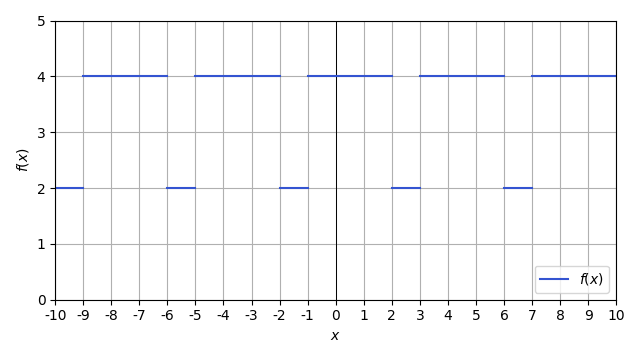
\includegraphics[width=0.7\textwidth]{square_wave/func.png}
    \caption{График функции $f(t)$}
\end{figure}

Итак, период функции $f(t)$ равен $T = 4 \ \Rightarrow\  \omega_n = \nicefrac{2\pi n}{4}$. Пришло время найти коэффициенты Фурье для этой функции --- вычислим первые три $a_n$, $b_n$ и $c_n$ ручками.

$$a_0 = \frac{2}{4} \left( \int_{2}^{3} 2 dt + \int_{3}^{6} 4 dt \right) = \frac{2}{4}\left( 2t\at^3_2 + 4t\at^6_3 \right) = \frac{2}{4}\left( 6 - 4 + 24 - 12 \right) = \msquared{\frac{14}{2}}$$

$$a_1 = \frac{2}{4}\left( \int_{2}^{3} 2\cos\frac{2\pi t}{4}\,dt + \int_{3}^{6} 4\cos\frac{2\pi t}{4}\,dt \right) = \frac{2}{4}\left( \frac{4\sin \frac{\pi t}{2}}{\pi}\at^3_2 + \frac{8\sin\frac{\pi t}{2}}{\pi}\at^6_3\right) = \frac{2}{4}\left(\frac{-4}{\pi} +\frac{8}{\pi} \right) = \msquared{\frac{2}{\pi}}$$

$$a_2 = \frac{2}{4}\left( \int_{2}^{3} 2\cos\frac{4\pi t}{4}\,dt + \int_{3}^{6} 4\cos\frac{4\pi t}{4}\,dt \right) = \frac{2}{4}\left( \frac{4\sin \pi t}{2\pi}\at^3_2 + \frac{8\sin\pi t}{2\pi}\at^6_3\right) = \frac{2}{4}\left(0 - 0 \right) = \msquared{0}$$

Теперь найдём коэффициенты $b_n$:

$$b_1 = \frac{2}{4}\left( \int_{2}^{3} 2\sin\frac{2\pi t}{4}\,dt + \int_{3}^{6} 4\sin\frac{2\pi t}{4}\,dt \right) = -\frac{2}{4}\left( \frac{4\cos\frac{2\pi t}{4}}{\pi}\at_2^3 + \frac{8\cos \frac{2\pi t}{4}}{\pi}\at_3^6 \right) = \frac{2}{4}\left(\frac{-4}{\pi} + \frac{8}{\pi}\right) = \msquared{\frac{2}{\pi}}$$

$$b_2 = \frac{2}{4}\left( \int_{2}^{3} 2\sin\frac{4\pi t}{4}\,dt + \int_{3}^{6} 4\sin\frac{4\pi t}{4}\,dt \right) = -\frac{2}{4}\left( \frac{2\cos\pi t}{\pi}\at_2^3 + \frac{4\cos \pi t}{\pi}\at_3^6 \right) = \frac{2}{4}\left(\frac{4}{\pi} - \frac{8}{\pi}\right) =\msquared{-\frac{2}{\pi}}$$

На очереди коэффициенты $c_n$:
$$c_0 = \frac{1}{4}\left( \int_{2}^{3} 2\,dt + \int_{3}^{6} 4\,dt \right) = \frac{a_0}{2} = \msquared{\frac{14}{4}}$$

$$c_1 = \frac{1}{4}\left( \int_{2}^{3} 2\e^{-\frac{2\pi it}{2}}\,dt + \int_{3}^{6} 4\e^{-\frac{2 \pi it}{2}}\,dt \right) = \frac{\frac{2}{\pi}-\frac{2}{\pi}i}{2} = \frac{1}{\pi} - \frac{i}{\pi} = \msquared{0.318 - 0.318i}$$

$$c_{-1} = \frac{1}{4}\left( \int_{2}^{3} 2\e^{\frac{2\pi it}{2}}\,dt + \int_{3}^{6} 4\e^{\frac{2 \pi it}{2}}\,dt \right) = \frac{\frac{2}{\pi}+\frac{2}{\pi}i}{2} = \frac{1}{\pi} + \frac{i}{\pi} = \msquared{0.318 + 0.318i}$$

$$c_2 = \frac{1}{4}\left( \int_{2}^{3} 2\e^{-\frac{4\pi it}{2}}\,dt + \int_{3}^{6} 4\e^{-\frac{4\pi it}{2}}\,dt \right) = \frac{0 + \frac{2}{\pi}i}{2} = 0 + \frac{i}{\pi} = \msquared{0 + 0.318i}$$

$$c_{-2} = \frac{1}{4}\left( \int_{2}^{3} 2\e^{\frac{4\pi it}{2}}\,dt + \int_{3}^{6} 4\e^{\frac{4\pi it}{2}}\,dt \right) = \frac{0 - \frac{2}{\pi}i}{2} = 0 - \frac{i}{\pi} = \msquared{0 - 0.318i}$$

Для проверки напишем программу, которая вычисляет коэффициенты Фурье для любого $n$.
\begin{lstlisting}[language=Python, caption=Вычисление коэффициентов Фурье]
import numpy as np

T = 4

def f(t):
    """Функция, для которой вычисляются коэффициенты Фурье."""
    return np.vectorize(lambda t: 2 if 1 <= (t - 1) % 4 < 2 else 4)(t)

def a(n, func=f, s=(-T / 2), p=T):
    """Вычисляет коэффициент a_n для функции func на отрезке (s, s + p)."""
    return 2 / p * dot_product(func, lambda t: np.cos(w(p) * n * t), s, s + p)

def b(n, func=f, s=(-T / 2), p=T):
    """Вычисляет коэффициент b_n для функции func на отрезке (s, s + p)."""
    return 2 / p * dot_product(func, lambda t: np.sin(w(p) * n * t), s, s + p)

def c(n, func=f, s=(-T / 2), p=T):
    """Вычисляет коэффициент c_n для функции func на отрезке (s, s + p)."""
    return 1 / p * dot_product(func, lambda t: np.exp(-1j * w(p) * n * t), s, s + p)

def dot_product(f, g, a, b):
    """Вычисляет скалярное произведение функций f и g на отрезке [a, b]."""
    x = np.linspace(a, b, 10000)
    dx = x[1] - x[0]
    return np.dot(f(x), g(x)) * dx

def coefficients(n):
    """Вычисляет коэффициенты Фурье a_n, b_n и c_n для функции f с периодом T."""
    return a(n).round(3), b(n).round(3), c(n).round(3), c(-n).round(3)

coef_num = int(data) if (data := input('Номер коэффициента: ')) else None
w = lambda period: 2 * np.pi / period
for n in range(0, coef_num + 1):
    a_n, b_n, c_n, c_mn = coefficients(n)
    print(f'a_{n} = {a_n},\tb_{n} = {b_n},\tc_{n} = {c_n}  c_{-n} = {c_mn}')    
\end{lstlisting}

Выведем первые четыре коэффициента Фурье для функции $f(t)$ для проверки скрипта:
\begin{lstlisting}[caption=Вывод программы]
a_0 = 7.0,	b_0 = 0.0,	c_0 = (3.5+0j)  c_0 = (3.5+0j)
a_1 = 0.636,	b_1 = 0.637,	c_1 = (0.318-0.318j)  c_-1 = (0.318+0.318j)
a_2 = 0.0,	b_2 = -0.637,	c_2 = 0.318j  c_-2 = -0.318j
a_3 = -0.212,	b_3 = 0.212,	c_3 = (-0.106-0.106j)  c_-3 = (-0.106+0.106j)
\end{lstlisting}
Как можно заметить коэффициенты посчитанные руками и коэффициенты посчитанные программой равны, следовательно, мы делаем вывод о корректной работе и можем продолжать работу.

Воспользуемся этими коэффициентами для построения графиков тригонометрического $F_n$ и экспоненциального $G_n$ рядов Фурье для функции $f(t)$:
\begin{figure}[H]
    \centering
    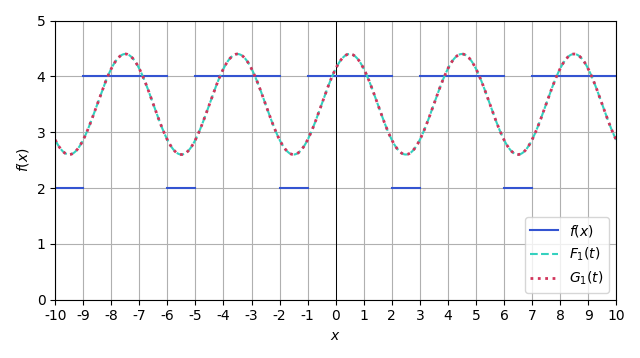
\includegraphics[width=0.7\linewidth]{square_wave/Im1.png}
    \caption{$n = 1$}
\end{figure}
\begin{figure}[H]
    \centering
    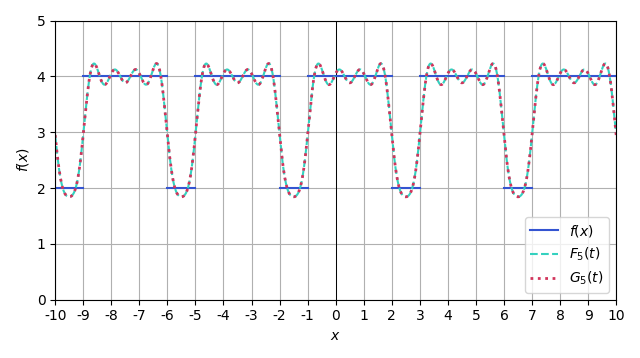
\includegraphics[width=0.7\linewidth]{square_wave/Im5.png}
    \caption{$n = 5$}
\end{figure}
\begin{figure}[H]
    \centering
    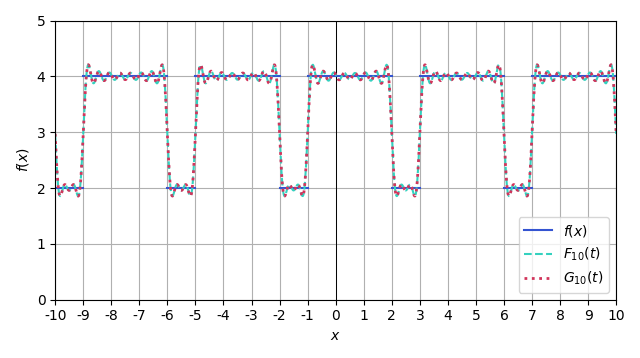
\includegraphics[width=0.7\linewidth]{square_wave/Im10.png}
    \caption{$n = 10$}
\end{figure}
\begin{figure}[H]
    \centering
    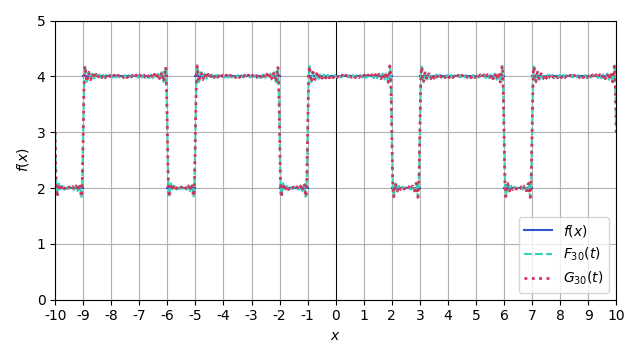
\includegraphics[width=0.7\linewidth]{square_wave/Im30.png}
    \caption{$n = 30$}
\end{figure}
\begin{figure}[H]
    \centering
    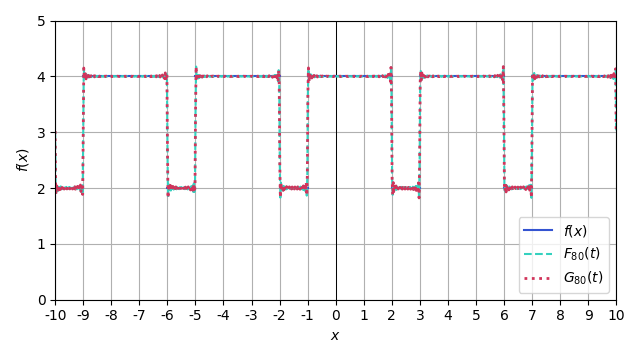
\includegraphics[width=0.7\linewidth]{square_wave/Im80.png}
    \caption{$n = 80$}
\end{figure}

Как мы видим, ряды Фурье $F_n(t)$ и $G_n(t)$ совпадают и вполне неплохо аппроксимируют функцию $f(t)$ уже при $n = 10$

Чтобы убедиться в том, что ряд Фурье действительно хорошо приближается к функции $f(t)$, проверим равенство Парсеваля при $n=80$ и при $n = 1$ --- так мы увидим разницу. Для этого напишем небольшую функцию для проверки равенства:

\begin{lstlisting}[language=Python, caption=Проверка равенства Парсеваля]
N = 1

def parseval_check():
    abs_func = np.vectorize(lambda x: abs(f(x)))
    norm_squared = dot_product(abs_func, abs_func, -np.pi, np.pi)
    
    a_coeffs = [a(i, abs_func, -np.pi, 2 * np.pi) for i in range(0, N + 1)]
    b_coeffs = [b(i, abs_func, -np.pi, 2 * np.pi) for i in range(0, N + 1)]
    c_coeffs = [c(i, abs_func, -np.pi, 2 * np.pi) for i in range(-N, N + 1)]
    ab_sum = np.pi * (a_coeffs[0] ** 2 / 2 + sum([a_coeffs[i] ** 2 + b_coeffs[i] ** 2 for i in range(1, N + 1)]))
    c_sum = 2 * np.pi * sum(abs(c_coeffs[i]) ** 2 for i in range(len(c_coeffs)))
    
    return abs(norm_squared - ab_sum), abs(norm_squared - c_sum)   


print(
    '||f|^2 - sum(|a_i|^2 + |b_i|^2)| = {:.5f}\n'
    '||f|^2 - sum(|c_i|^2)|           = {:.5f}'.format(*parseval_check())
    )
\end{lstlisting}
Посмотрим, что вывела программа: 

\begin{minipage}{0.48\textwidth}
\begin{lstlisting}[caption={Равенство Парсеваля при $n=1$}]
Parseval deviation:
||f|^2 - sum(|a_i|^2 + |b_i|^2)| = 4.63817
||f|^2 - sum(|c_i|^2)|           = 4.63817
\end{lstlisting}
\end{minipage}\hfill
\begin{minipage}{0.48\textwidth}
\begin{lstlisting}[caption={Равенство Парсеваля при $n=80$}, numbers=none]
||f|^2 - sum(|a_i|^2 + |b_i|^2)| = 0.05216
||f|^2 - sum(|c_i|^2)|           = 0.05216
\end{lstlisting}
\end{minipage}
Мы видим, что при увеличении числа коэффициентов в равенстве Парсеваля отклонение стремится к нулю. Можно сделать вывод, что ряд Фурье действительно приближается к функции $f(t)$ всё лучше и лучше с увеличением числа коэфициентов.

\subsection{Чётная функция}
Далее рассмотрим \textbf{четную периодическую функцию}: $f_\text{чет}(t) = |3\sin(2t)|$ на промежутке $\left[0, \frac{\pi}{2}\right]$. Построим график этой функции:
\begin{figure}[H]
    \centering 
    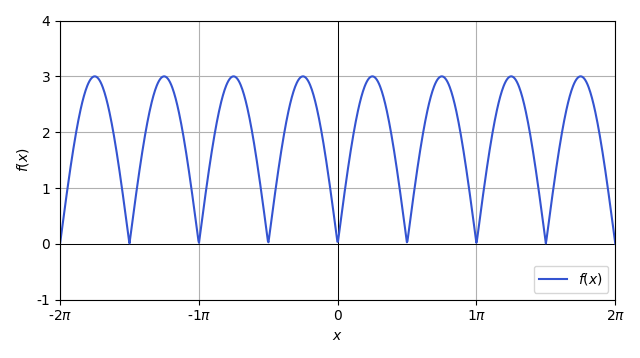
\includegraphics[width=0.7\textwidth]{even/func.png}
    \caption{График функции $f_\text{чет}(t)$}
\end{figure}

Период функции $f_\text{чет}(t)$ равен $T=\frac{\pi}{2}$, следовательно $\omega=4n$.
Чётность функции означает, что её разложение в ряд Фурье содержит только косинусные члены, а коэффициенты $b_n$ при синусах равны нулю. Таким образом, коэффициенты $a_n$ и $c_n$ в общем виде вычисляются следующим образом:
$$a_n = \frac{4}{\pi}\int_{0}^{\frac{\pi}{2}} |3\sin (2t)|\cos 4nt\,dt\qquad c_n = \frac{2}{\pi}\int_{0}^{\frac{\pi}{2}}|3\sin (2t)|\e^{-4int}\,dt$$
Упростим формулы:
$$a_n \;=\; \frac{4}{\pi}\int_{0}^{\tfrac{\pi}{2}}
   \bigl|2\,\sin(2t)\bigr|\;\cos(4nt)\,\mathrm{d}t
\;=\;
\frac{8}{\pi}\int_{0}^{\tfrac{\pi}{2}} \sin(2t)\,\cos(4nt)\,\mathrm{d}t = \;\frac{8}{\pi}\cdot \frac12 \biggl[\int_{0}^{\tfrac{\pi}{2}}\! \sin\bigl((4n+2)\,t\bigr)\,\mathrm{d}t + $$
$$+\int_{0}^{\tfrac{\pi}{2}}\! \sin\bigl((2-4n)\,t\bigr)\,\mathrm{d}t \biggr] =\;\frac{8}{\pi}\cdot \frac12\Bigl(\tfrac{2}{4n+2}+\tfrac{2}{2-4n}\Bigr)=\;\frac{8}{\pi}\cdot\frac{4}{\,(4n+2)(2-4n)\,}=$$
$$=\frac{8}{\pi}\cdot \frac{1}{\,1 - 4n^2\,}=\;\boxed{\;\frac{8}{\,\pi\,\bigl(1 - 4n^2\bigr)}.}$$

$$c_n\;=\; \frac{2}{\pi}\int_{0}^{\tfrac{\pi}{2}}\bigl|2\,\sin(2t)\bigr|\;e^{-4i\,n\,t}\,\mathrm{d}t\;=\; \frac{4}{\pi}\int_{0}^{\tfrac{\pi}{2}}  \sin(2t)\;e^{-4i\,n\,t}\,\mathrm{d}t=\;\frac{4}{\pi}\;\cdot\;\frac{1}{2i}\Bigl[\int_{0}^{\tfrac{\pi}{2}} e^{\,i(2 - 4n)\,t}\,\mathrm{d}t -$$
$$-\int_{0}^{\tfrac{\pi}{2}} e^{-\,i(4n + 2)\,t}\,\mathrm{d}t\Bigr] = \frac{4}{\pi}\,\cdot\frac{1}{\,1 - 4n^2\,}=\;\boxed{\;\frac{4}{\,\pi\,\bigl(1 - 4n^2\bigr)}.}$$



Изменим программу, которая вычисляет коэффициенты Фурье для любого $n$, под нашу функцию.
\begin{lstlisting}[language=Python, caption={Вычисление коэффициентов Фурье для функции $f_\text{чет}(t)$}]
...
def f(x):
    """Функция, для которой вычисляются коэффициенты Фурье."""
    return np.vectorize(lambda t: abs(3*np.sin(2 * t)))(x)
...   
\end{lstlisting}
Выведем первые четыре коэффициента Фурье, среди которых есть и необходимые по заданию $a_2$, $b_2$ и $c_2$:
\begin{lstlisting}[caption=Вывод программы]
a_0 = 2.547,    b_0 = 0.0,      c_0 = (1.273+0j)  c_0 = (1.273+0j)
a_1 = -0.849,   b_1 = 0.0,      c_1 = (-0.425+0j)  c_-1 = (-0.425-0j)
a_2 = -0.169,   b_2 = -0.0,     c_2 = (-0.085+0j)  c_-2 = (-0.085-0j)
a_3 = -0.073,   b_3 = -0.0,     c_3 = (-0.037-0j)  c_-3 = (-0.037+0j)
\end{lstlisting}
Убеждаемся, что, действительно, коэффициенты $b_n$ равны нулю. Теперь сделаем графики. Воспользуемся этими коэффициентами для построения тригонометрического $F_n$ и экспоненциального $G_n$ рядов Фурье для функции $f_\text{чет}(t)$:
\begin{figure}[H]
    \centering
    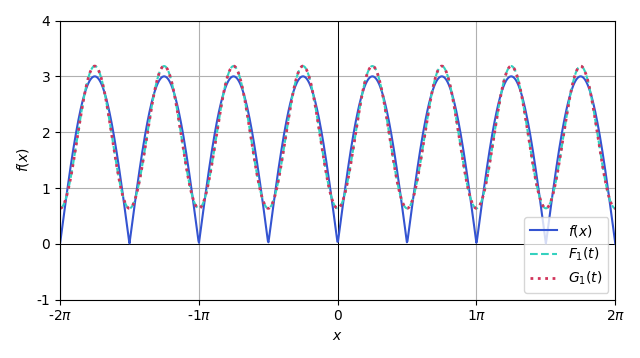
\includegraphics[width=0.7\linewidth]{even/Im1.png}
    \caption{$n = 1$}
\end{figure}
\begin{figure}[H]
    \centering
    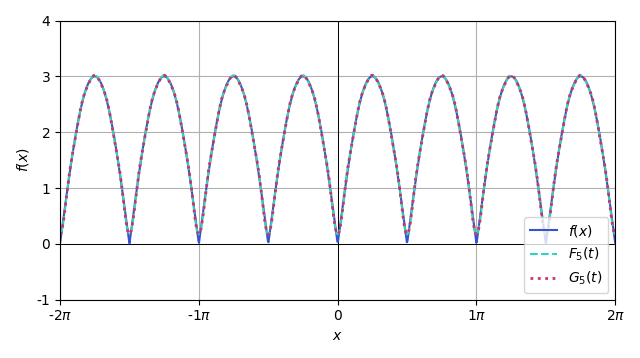
\includegraphics[width=0.7\linewidth]{even/Im5.png}
    \caption{$n = 5$}
\end{figure}
\begin{figure}[H]
    \centering
    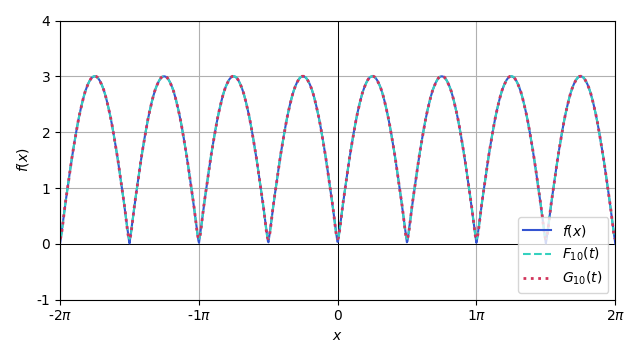
\includegraphics[width=0.7\linewidth]{even/Im10.png}
    \caption{$n = 10$}
\end{figure}
\begin{figure}[H]
    \centering
    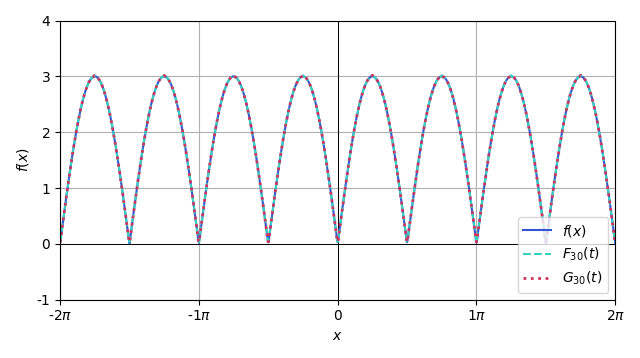
\includegraphics[width=0.7\linewidth]{even/Im30.png}
    \caption{$n = 30$}
\end{figure}
\begin{figure}[H]
    \centering
    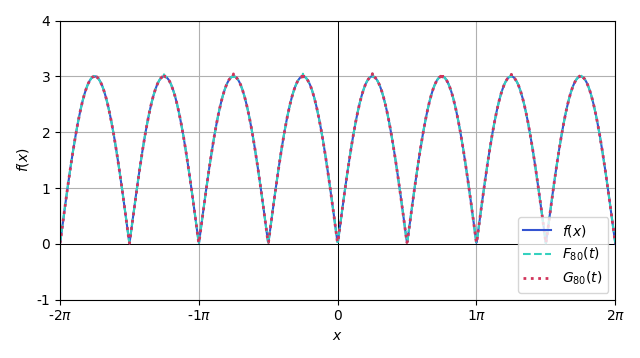
\includegraphics[width=0.7\linewidth]{even/Im80.png}
    \caption{$n = 80$}
\end{figure}

Видно, что даже при небольших $n$ приближение довольно точное, а при увеличении числа гармоник аппроксимация становится практически неотличимой от оригинала. Разложение чётной функции в ряд Фурье содержит только косинусные члены, так как синусные члены отвечают за нечётную компоненту. В отличие от функций с разрывами, у данной функции нет эффекта Гиббса, что делает её аппроксимацию более гладкой.

Чтобы убедиться в том, что при $n = 80$ ряд Фурье действительно аппроксимирует функцию $f_\text{чет}(t)$ довольно точно, проверим равенство Парсеваля при этом же количестве коэффициентов и при $n = 1$ --- так мы увидим разницу.

\begin{minipage}{0.48\textwidth}
\begin{lstlisting}[caption={Равенство Парсеваля при $n=1$}]
||f|^2 - sum(|a_i|^2 + |b_i|^2)| = 5.35602
||f|^2 - sum(|c_i|^2)|           = 5.35602
\end{lstlisting}
\end{minipage}\hfill
\begin{minipage}{0.48\textwidth}
\begin{lstlisting}[caption={Равенство Парсеваля при $n=80$}, numbers=none]
||f|^2 - sum(|a_i|^2 + |b_i|^2)| = 0.00011
||f|^2 - sum(|c_i|^2)|           = 0.00011
\end{lstlisting}
\end{minipage}
Мы наблюдаем, что отклонение в равенстве Парсеваля с увеличением количества коэффициентов стремится к нулю. Это означает, что ряд Фурье действительно приближается к функции $f_\text{чет}(t)$ всё лучше и лучше.

\subsection{Нечётная функция}
Теперь рассмотрим \textbf{Нечётную  периодическую функцию}: $$f_\text{неч}(t) =((t-3) \mod 6 - 3)$$ на промежутке $\left[-3, 3\right]$. Построим график этой функции:
\begin{figure}[H]
    \centering 
    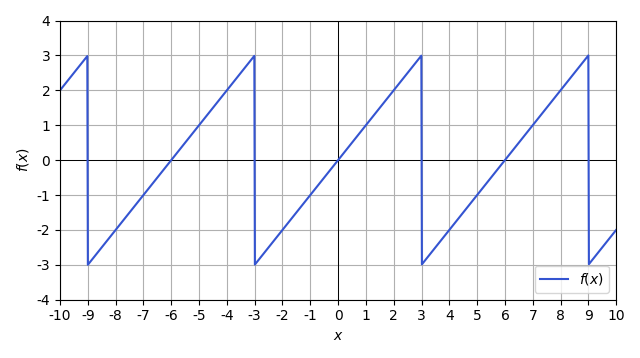
\includegraphics[width=0.7\textwidth]{odd/func.png}
    \caption{График функции $f_\text{чет}(t)$}
\end{figure}

Период функции $f_\text{неч}(t)$ равен $T=6$, следовательно $\omega=\frac{\pi n}{3}$. Вновь найдём коэффициенты Фурье для функции с помощью уже написанной нами ранее программы, но перед этим посмотрим на интегралы. Для нечётной функции $f_\text{неч}(t)$ коэффициенты $a_n$ равны нулю и ряд Фурье строится по синусам. Таким образом, коэффициенты $b_n$ и $c_n$ в общем виде вычисляются следующим образом:
$$b_n = \frac{1}{3}\int_{-3}^{3} \left( (t - 3) \bmod 6 - 3 \right)\sin \frac{n\pi t}{3}\,dt\qquad c_n = \frac{1}{6}\int_{-3}^{3}\left( (t - 3) \bmod 6 - 3 \right)\e^{\frac{-in\pi t}{3}}\,dt$$

\[
\text{На отрезке }[-3,3]:
\quad
((t-3)\bmod6)\,-\,3 = t \quad\Longrightarrow
\]
$$b_n=\frac{1}{3}\int_{-3}^{3}t\,\sin\!\Bigl(\!\tfrac{n\pi t}{3}\Bigr)\,dt = \frac{5}{n\,\pi}\,\bigl(-1\bigr)^{\,n+1},$$
$$c_n=\frac{1}{6}\int_{-3}^{3}t\,\exp^{\frac{-in\pi t}{3}}\,dt = i\,\frac{5}{2\,n\,\pi}\,\bigl(-1\bigr)^{\,n}$$


Изменим программу, которая вычисляет коэффициенты Фурье для любого $n$, под нашу функцию.
\begin{lstlisting}[language=Python, caption={Вычисление коэффициентов Фурье для функции $f_\text{неч}(t)$}]
...
def f(x):
    """Функция, для которой вычисляются коэффициенты Фурье."""
    return np.vectorize(lambda t: ((t - 3) % 6 - 3))(x)
...   
\end{lstlisting}
Выведем первые четыре коэффициента Фурье и убедимся в отсутсвии $cos(t)$ в разложении: 
\begin{lstlisting}[caption=Вывод программы]
a_0 = 0.0,	b_0 = 0.0,	c_0 = 0j  c_0 = 0j
a_1 = -0.0,	b_1 = 1.592,	c_1 = (-0-0.796j)  c_-1 = (-0+0.796j)
a_2 = 0.0,	b_2 = -0.796,	c_2 = 0.398j  c_-2 = -0.398j
a_3 = -0.0,	b_3 = 0.531,	c_3 = (-0-0.265j)  c_-3 = (-0+0.265j)
\end{lstlisting}
С помошью программы находим коэффициенты при больших значениях $n$ и строим соответсвующие графики тригонометрической функции $F_n$ и экспоненциальной $G_n$ рядов Фурье для функции $f_\text{неч}(t)$:
\begin{figure}[H]
    \centering
    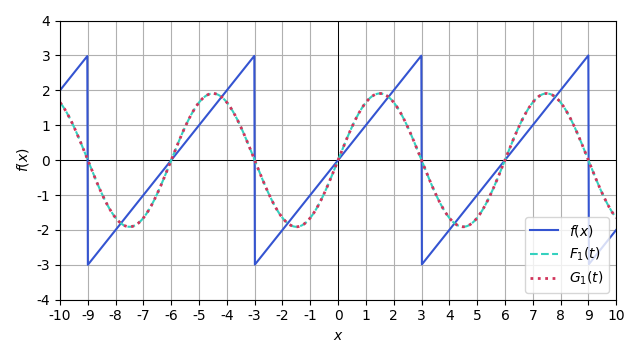
\includegraphics[width=0.7\linewidth]{odd/Im1.png}
    \caption{$n = 1$}
\end{figure}
\begin{figure}[H]
    \centering
    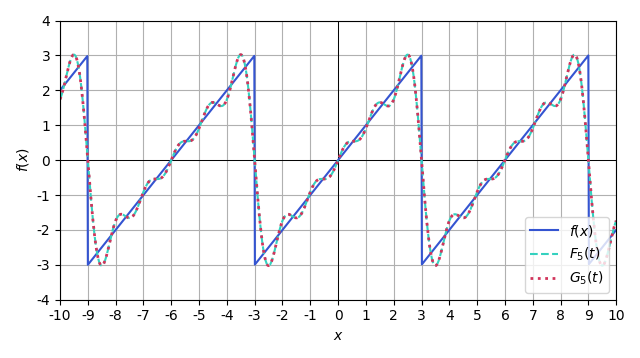
\includegraphics[width=0.7\linewidth]{odd/Im5.png}
    \caption{$n = 5$}
\end{figure}
\begin{figure}[H]
    \centering
    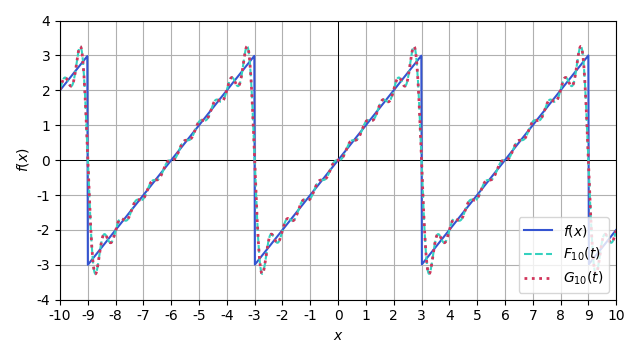
\includegraphics[width=0.7\linewidth]{odd/Im10.png}
    \caption{$n = 10$}
\end{figure}
\begin{figure}[H]
    \centering
    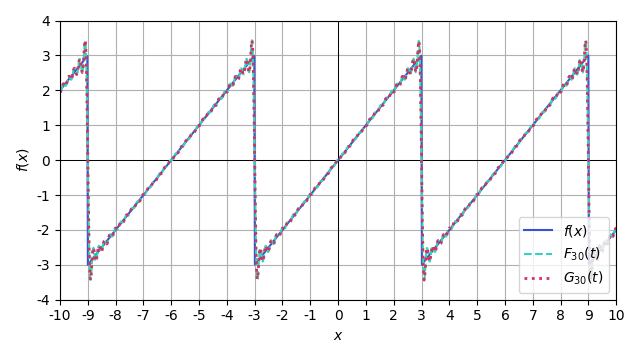
\includegraphics[width=0.7\linewidth]{odd/Im30.png}
    \caption{$n = 30$}
\end{figure}
\begin{figure}[H]
    \centering
    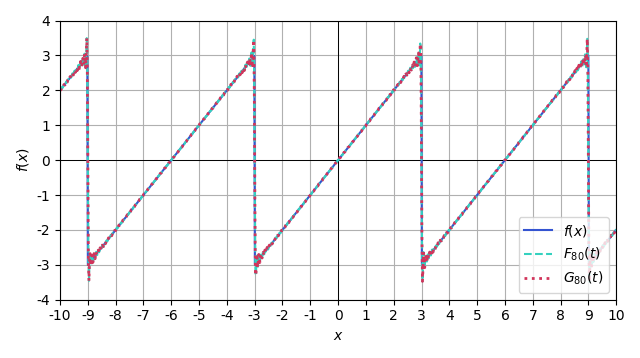
\includegraphics[width=0.7\linewidth]{odd/Im80.png}
    \caption{$n = 80$}
\end{figure}

Графики рядов Фурье $F_n(x)$ и $G_n(x)$ совпадают и хорошо приближаются к функции $f(x)$ при $n > 10$. Также не наблюдается эффекта Гиббса.
Чтобы убедиться в том, что при $n = 80$ ряд Фурье действительно аппроксимирует функцию $f_\text{неч}(t)$ довольно точно, проверим равенство Парсеваля при $n = 80$ и при $n = 1$:

\begin{minipage}{0.48\textwidth}
\begin{lstlisting}[caption={Равенство Парсеваля при $n=1$}]
||f|^2 - sum(|a_i|^2 + |b_i|^2)| = 0.05630
||f|^2 - sum(|c_i|^2)|           = 0.05630
\end{lstlisting}
\end{minipage}\hfill
\begin{minipage}{0.48\textwidth}
\begin{lstlisting}[caption={Равенство Парсеваля при $n=80$}, numbers=none]
||f|^2 - sum(|a_i|^2 + |b_i|^2)| = 0.00524
||f|^2 - sum(|c_i|^2)|           = 0.00524
\end{lstlisting}
\end{minipage}
Мы наблюдаем, что отклонение в равенстве Парсеваля с увеличением количества коэффициентов стремится к нулю. Это означает, что ряд Фурье действительно приближается к функции $f_\text{чет}(t)$ всё лучше и лучше.

\subsection{Общая периодическая функция}
И наконец рассмотрим \textbf{Общую периодическую функцию}: $$f_\text{об}(t) =\sqrt{4 - ((t - 1) \mod 2)^2}$$ на промежутке $\left[-1, 1\right]$. Она не является ни четной, ни нечетной. Построим график этой функции:
\begin{figure}[H]
    \centering 
    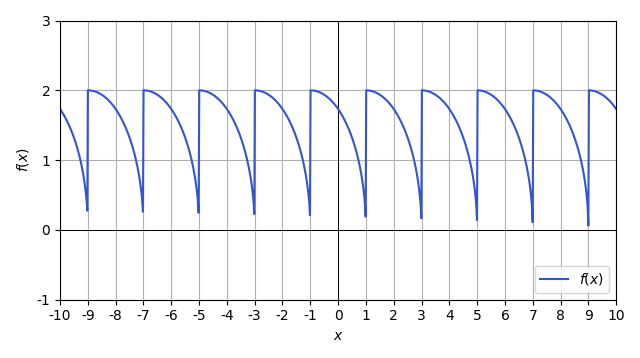
\includegraphics[width=0.7\textwidth]{per/func.png}
    \caption{График функции $f_\text{чет}(t)$}
\end{figure}

Период функции $f_\text{об}(t)$ равен $T=2 \Rightarrow \omega=\pi n$. 
Взглянем на то, как вычисляются коэффициенты $a_n$, $b_n$ и $c_n$ в общем виде:
$$a_n = \frac{2}{2}\int_{-1}^{1} \sqrt{4 - ((t - 1) \mod 2)^2}\sin \pi nt\,dt$$
$$b_n = \frac{2}{2}\int_{-1}^{1} \sqrt{4 - ((t - 1) \mod 2)^2}\cos \pi nt\,dt$$  
$$c_n = \frac{1}{2}\int_{-1}^{1}\sqrt{4 - ((t - 1) \mod 2)^2}\e^{-i\pi nt}\,dt$$    

Далее изменим программу, которая вычисляет коэффициенты Фурье, под функцию $f_\text{об}(t)$.
\begin{lstlisting}[language=Python, caption={Вычисление коэффициентов Фурье для функции $f_\text{об}(t)$}]
...
def f(x):
    """Функция, для которой вычисляются коэффициенты Фурье."""
    return np.vectorize(lambda t: (4 - ((t - 1) % 2)**2) ** (1/2))(x)
...   
\end{lstlisting}

Выведем первые четыре коэффициента Фурье: 
\begin{lstlisting}[caption=Вывод программы]
a_0 = 3.142,	b_0 = 0.0,	c_0 = (1.571+0j)  c_0 = (1.571+0j)
a_1 = 0.212,	b_1 = -0.413,	c_1 = (0.106+0.206j)  c_-1 = (0.106-0.206j)
a_2 = -0.077,	b_2 = 0.238,	c_2 = (-0.038-0.119j)  c_-2 = (-0.038+0.119j)
a_3 = 0.042,	b_3 = -0.169,	c_3 = (0.021+0.084j)  c_-3 = (0.021-0.084j)
\end{lstlisting}

Программно найдем коэффициенты при больших значениях $n$ и построим соответсвующие графики тригонометрической функции $F_n$ и экспоненциальной $G_n$ рядов Фурье для функции $f_\text{об}(t)$:
\begin{figure}[H]
    \centering
    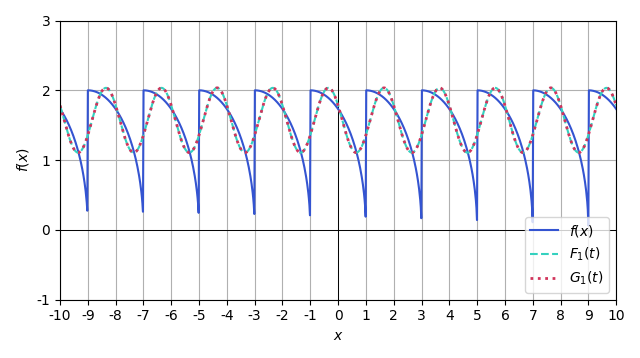
\includegraphics[width=0.7\linewidth]{per/Im1.png}
    \caption{$n = 1$}
\end{figure}
\begin{figure}[H]
    \centering
    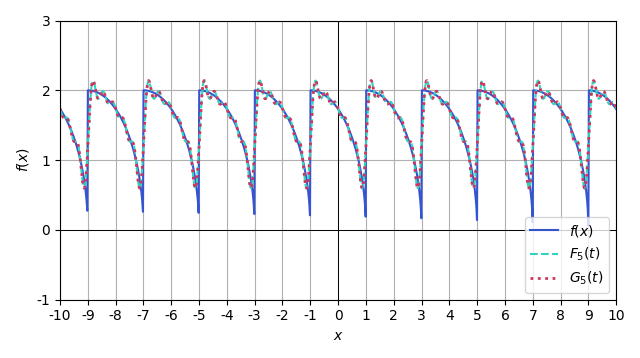
\includegraphics[width=0.7\linewidth]{per/Im5.png}
    \caption{$n = 5$}
\end{figure}
\begin{figure}[H]
    \centering
    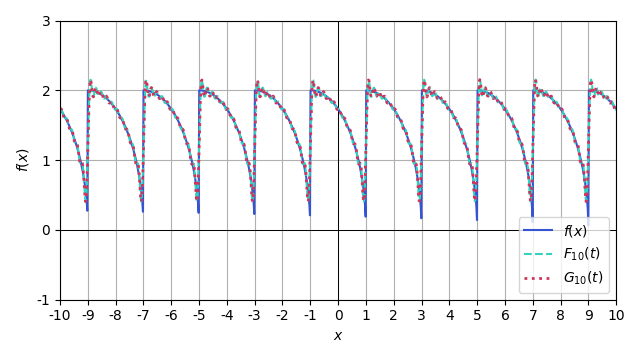
\includegraphics[width=0.7\linewidth]{per/Im10.png}
    \caption{$n = 10$}
\end{figure}
\begin{figure}[H]
    \centering
    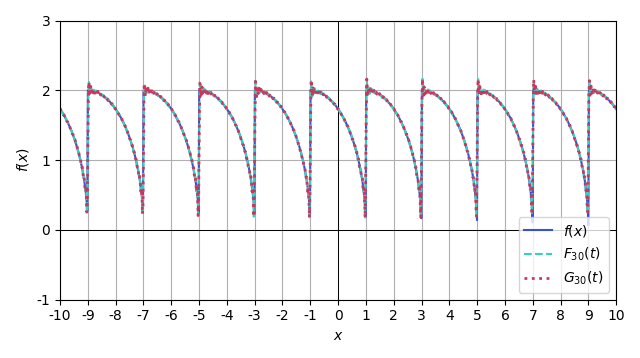
\includegraphics[width=0.7\linewidth]{per/Im30.png}
    \caption{$n = 30$}
\end{figure}
\begin{figure}[H]
    \centering
    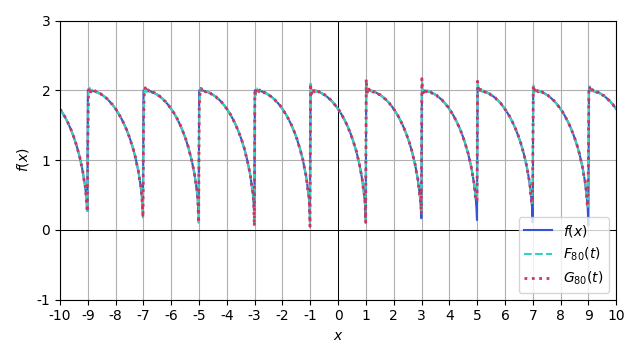
\includegraphics[width=0.7\linewidth]{per/Im80.png}
    \caption{$n = 80$}
\end{figure}

Графики рядов Фурье $F_n(x)$ и $G_n(x)$ совпадают и хорошо приближаются к функции $f(x)$.
Проверим равенство Парсеваля для $n = 80$ и $n = 1$:

\begin{minipage}{0.48\textwidth}
\begin{lstlisting}[caption={Равенство Парсеваля при $n=1$}]
||f|^2 - sum(|a_i|^2 + |b_i|^2)| = 1.38261
||f|^2 - sum(|c_i|^2)|           = 1.38261
\end{lstlisting}
\end{minipage}\hfill
\begin{minipage}{0.48\textwidth}
\begin{lstlisting}[caption={Равенство Парсеваля при $n=80$}, numbers=none]
||f|^2 - sum(|a_i|^2 + |b_i|^2)| = 0.06085
||f|^2 - sum(|c_i|^2)|           = 0.06085
\end{lstlisting}
\end{minipage}
Мы наблюдаем, что отклонение в равенстве Парсеваля с увеличением количества коэффициентов стремится к нулю. Это означает, что ряд Фурье действительно приближается к функции $f_\text{чет}(t)$ всё лучше и лучше.

\section{Задание 2. Комплексная функция}
Для выполнения этого задания зададим $R = 2$ и $T = 4\ \Rightarrow\ \omega = \nicefrac{\pi n}{2}$. По условию получим следующую комплекснозначную функцию, заданную параметрическим образом:
$$\text{Re}\,f(t) = \begin{cases}
    2, & t \in [-\frac{1}{2}, \frac{1}{2}),\\
    4-4t, & t \in [\frac{1}{2}, \frac{3}{2}),\\
    -2, & t \in [\frac{3}{2}, \frac{5}{2}),\\
    -12+4t, & t \in [\frac{5}{2}, \frac{7}{2}),\\
\end{cases}\qquad\text{Im}\,f(t) = \begin{cases}
    4t, & t \in [-\frac{1}{2}, \frac{1}{2}),\\
    2, & t \in [\frac{1}{2}, \frac{3}{2}),\\
    8-4t, & t \in [\frac{3}{2}, \frac{5}{2}),\\
    -2, & t \in [\frac{5}{2}, \frac{7}{2}).\\
\end{cases}$$
Расмотрим график функции $f(t)$ на комплексной плоскости:
\begin{figure}[H]
    \centering 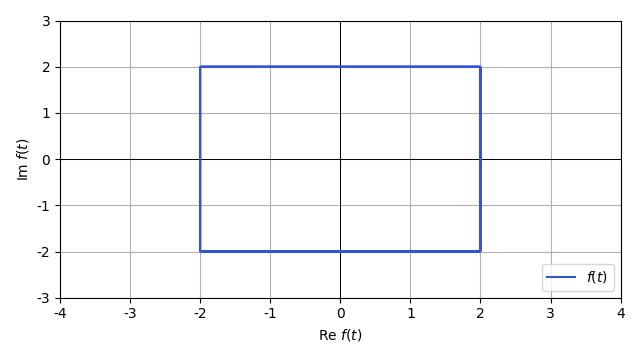
\includegraphics[width=0.7\textwidth]{param/func.png}
    \caption{График функции $f(t)$}
\end{figure}
Получаем вот такой квадрат на комплексной плоскости. Теперь найдём коэффициенты Фурье $c_n$ для этой функции, которые в общем виде вычисляются так:
$$c_n = \frac{1}{4}\int_{-1/2}^{7/2}f(t)e^{-i\frac{\pi n}{2}t}\,dt = \frac{1}{4}\left( \int_{-1/2}^{1/2} \left( 2 + 4ti \right)e^{-i\frac{\pi n}{2}t}\,dt + \int_{1/2}^{3/2}\left( 4 - 4t + 2i \right)e^{-i\frac{\pi n}{2}t}\,dt +  \right.$$
$$\left. + \int_{3/2}^{5/2}\left( -2 + (8 - 4t)i \right)e^{-i\frac{\pi n}{2}t}\,dt + \int_{5/2}^{7/2}\left( -12 + 4t -2i \right)e^{-i\frac{\pi n}{2}t}\,dt\right)$$
Вычислим вручную $c_0$, $c_1$, $c_2$:
$$c_0 = \frac{1}{4}\left( \int_{-1/2}^{1/2} \left( 2 + 4ti \right)\,dt + \int_{1/2}^{3/2}\left( 4 - 4t + 2i \right)\,dt + \int_{3/2}^{5/2}\left( -2 + (8 - 4t)i \right)\,dt + \int_{5/2}^{7/2}\left( -12 + 4t -2i \right)\,dt\right)$$
$$= \frac{1}{4}(2+2i-2-2i) = \msquared{0}$$
$$c_1 = \frac{1}{4}\left( \int_{-1/2}^{1/2} \left( 2 + 4ti \right)e^{-i\frac{\pi}{2}t}\,dt + \int_{1/2}^{3/2}\left( 4 - 4t + 2i \right)e^{-i\frac{\pi}{2}t}\,dt + \int_{3/2}^{5/2}\left( -2 + (8 - 4t)i \right)e^{-i\frac{\pi}{2}t}\,dt + \right.$$
$$\left.+ \int_{5/2}^{7/2}\left( -12 + 4t -2i \right)e^{-i\frac{\pi}{2}t}\,dt \right)=\msquared{2.293}$$

$$c_{-1} = \frac{1}{4}\left( \int_{-1/2}^{1/2} \left( 2 + 4ti \right)e^{i\frac{\pi}{2}t}\,dt + \int_{1/2}^{3/2}\left( 4 - 4t + 2i \right)e^{i\frac{\pi}{2}t}\,dt + \int_{3/2}^{5/2}\left( -2 + (8 - 4t)i)e^{i\frac{\pi}{2}t}\,dt + \right. \right.$$
$$\left.+ \int_{5/2}^{7/2}\left( -12 + 4t -2i \right)e^{i\frac{\pi}{2}t}\,dt \right)=\msquared{0}$$

$$c_2 = \frac{1}{4}\left( \int_{-1/2}^{1/2} \left( 2 + 4ti \right)e^{-i\pi t}\,dt + \int_{1/2}^{3/2}\left( 4 - 4t + 2i \right)e^{-i\pi t}\,dt + \int_{3/2}^{5/2}\left( -2 + (8 - 4t)i \right)e^{-i\pi t}\,dt + \right.$$
$$\left. + \int_{5/2}^{7/2}\left( -12 + 4t -2i \right)e^{-i\pi t}\,dt\right) = \msquared{0}$$

$$c_{-2} = \frac{1}{4}\left( \int_{-1/2}^{1/2} \left( 2 + 4ti \right)e^{i\pi t}\,dt + \int_{1/2}^{3/2}\left( 4 - 4t + 2i \right)e^{i\pi t}\,dt + \int_{3/2}^{5/2}\left( -2 + (8 - 4t)i \right)e^{i\pi t}\,dt + \right.$$
$$\left. + \int_{5/2}^{7/2}\left( -12 + 4t -2i \right)e^{i\pi t}\,dt\right) = \msquared{0}$$

Теперь воспользуемся программой, которая вычисляет коэффициенты Фурье для любого $n$. Программа уже написана, поэтому мы просто вставим в неё нашу функцию и запустим её, чтобы получить коэффициенты:
\begin{lstlisting}[language=Python, caption={Вычисление коэффициентов Фурье для функции $f(t)$}]
...
def f(x):
    def create_parametric_func(R, T):
        def pfunc_instance(t):
            t = (t + T / 8) % T - T / 8
            if -T / 8 <= t < T / 8:
                real = R
            elif T / 8 <= t < 3 * T / 8:
                real = 2 * R - 8 * R * t / T
            elif 3 * T / 8 <= t < 5 * T / 8:
                real = -R
            elif 5 * T / 8 <= t <= 7 * T / 8:
                real = -6 * R + 8 * R * t / T

            if -T / 8 <= t < T / 8:
                imag = 8 * R * t / T
            if T / 8 <= t < 3 * T / 8:
                imag = R
            if 3 * T / 8 <= t < 5 * T / 8:
                imag = 4 * R - 8 * R * t / T
            if 5 * T / 8 <= t <= 7 * T / 8:
                imag = -R

            return real + 1j * imag

        return pfunc_instance

    return create_parametric_func(2, 4)
...   
\end{lstlisting}
Итак, программа выдаёт нам первые 5 коэфцииентов:
\begin{lstlisting}[caption=Вывод программы]
c_0 = (-0-0j)       c_0 = (-0-0j)
c_1 = (2.293+0j)    c_-1 = -0j
c_2 = (-0-0j)       c_-2 = (-0-0j)
c_3 = -0j           c_-3 = (-0.255+0j)
\end{lstlisting}
Мы видим, что коэффициент $c_2$ равен нулю, как и большинство коэффициентов $c_n$ и $c_{-n}$.

Теперь построим графики для различных первых $n$ коэффициентов:
\begin{figure}[H]
    \centering
    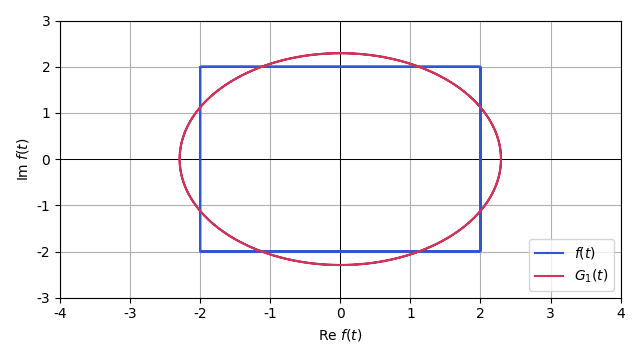
\includegraphics[width=0.8\linewidth]{param/1.png}
    \caption{$n = 1$}
\end{figure}
\begin{figure}[H]
    \centering
    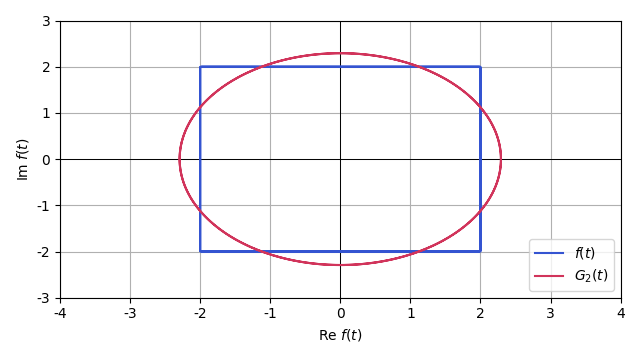
\includegraphics[width=0.8\linewidth]{param/2.png}
    \caption{$n = 2$}
\end{figure}
\begin{figure}[H]
    \centering
    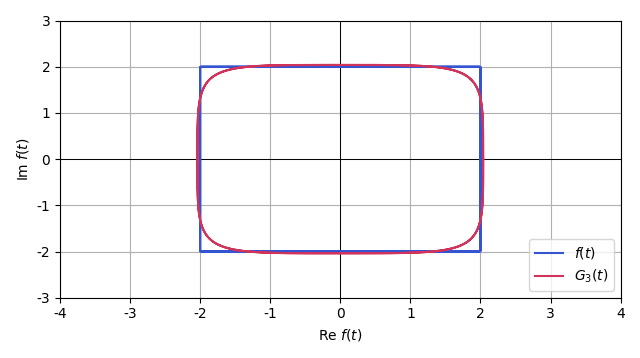
\includegraphics[width=0.8\linewidth]{param/3.png}
    \caption{$n = 3$}
\end{figure}
\begin{figure}[H]
    \centering
    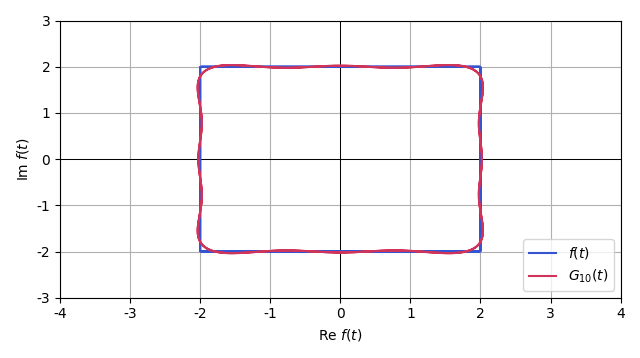
\includegraphics[width=0.8\linewidth]{param/10.png}
    \caption{$n = 10$}
\end{figure}
С первых значений, вокруг квадрата формируется круг, который с увеличением числа гармоник всё больше становится похож на квадрат. Теперь построим другие графики: на абсциссе отложим t, а по ординате отложим сначала вещественные части $f(t)$ и $G_n(t)$, а затем мнимые.
\begin{figure}[H]
    \centering
    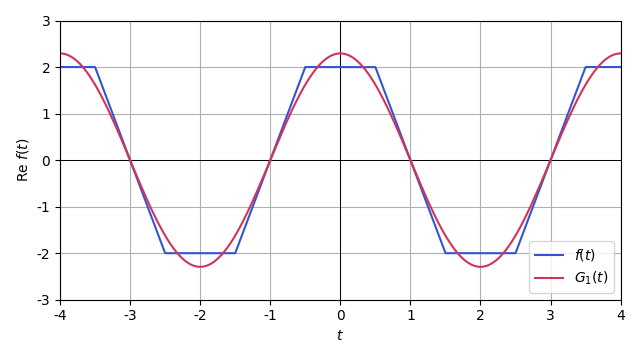
\includegraphics[width=0.7\linewidth]{param/Re1.png}
    \caption{$Re\quad n = 1$}
\end{figure}
\begin{figure}[H]
    \centering
    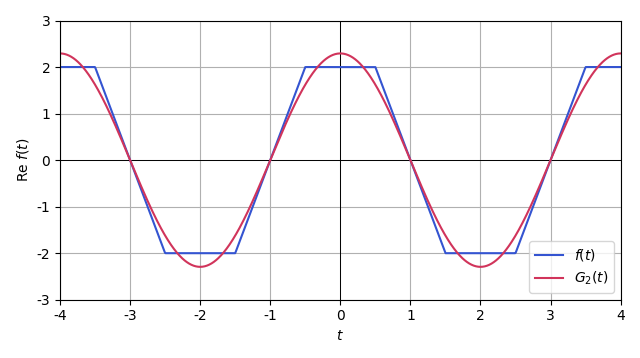
\includegraphics[width=0.7\linewidth]{param/Re2.png}
    \caption{$Re\quad n = 2$}
\end{figure}
\begin{figure}[H]
    \centering
    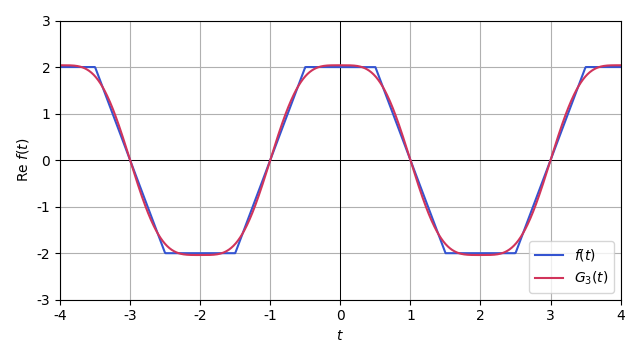
\includegraphics[width=0.7\linewidth]{param/Re3.png}
    \caption{$Re\quad n = 3$}
\end{figure}
\begin{figure}[H]
    \centering
    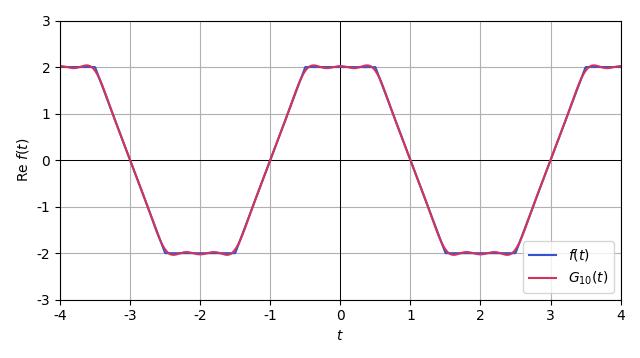
\includegraphics[width=0.7\linewidth]{param/Re10.png}
    \caption{$Re\quad n = 10$}
\end{figure}
\begin{figure}[H]
    \centering
    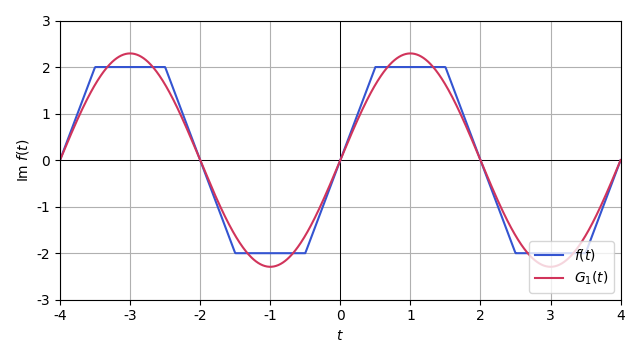
\includegraphics[width=0.7\linewidth]{param/Im1.png}
    \caption{$Im\quad n = 1$}
\end{figure}
\begin{figure}[H]
    \centering
    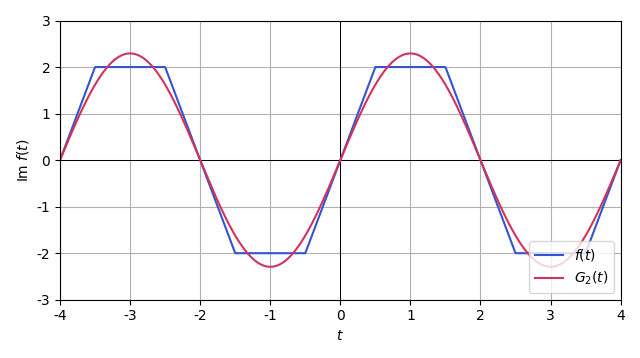
\includegraphics[width=0.7\linewidth]{param/Im2.png}
    \caption{$Im\quad n = 2$}
\end{figure}
\begin{figure}[H]
    \centering
    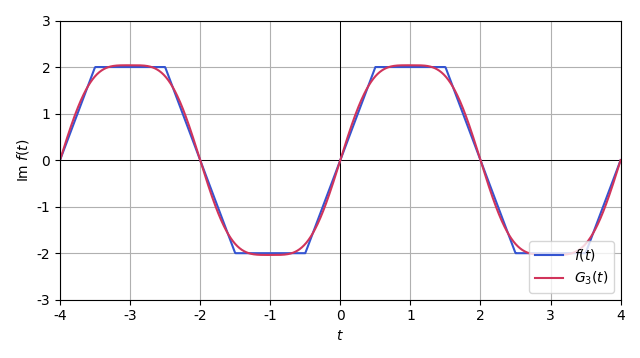
\includegraphics[width=0.7\linewidth]{param/Im3.png}
    \caption{$Im\quad n = 3$}
\end{figure}
\begin{figure}[H]
    \centering
    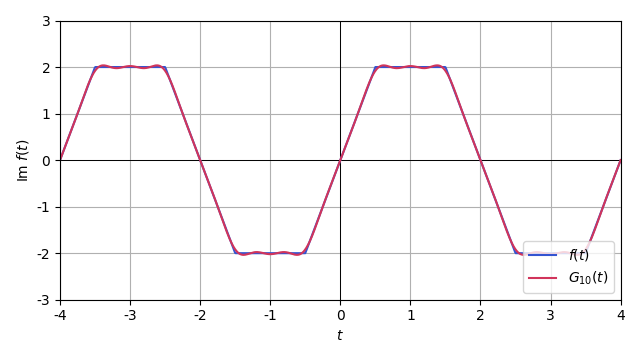
\includegraphics[width=0.7\linewidth]{param/Im10.png}
    \caption{$Im\quad n = 10$}
\end{figure}
Мы можем сделать вывод, что $G_n(t)$ приближает исходную функцию $f(t)$ в вещественной и мнимой частях. 
Чтобы убедиться в том, что при $n = 10$ ряд Фурье очень точен к функции $f(t)$, проверим равенство Парсеваля при этом же количестве коэффициентов и при $n = 1$ --- так мы увидим разницу.
\begin{minipage}{0.48\textwidth}
\begin{lstlisting}[caption={Равенство Парасеваля при $n=1$}]
||f|^2 - sum(|a_i|^2 + |b_i|^2)| = 0.39629
||f|^2 - sum(|c_i|^2)|           = 0.39629
\end{lstlisting}
\end{minipage}\hfill
\begin{minipage}{0.48\textwidth}
\begin{lstlisting}[caption={Равенство Парасеваля при $n=10$}, numbers=none]
||f|^2 - sum(|a_i|^2 + |b_i|^2)| = 0.01920
||f|^2 - sum(|c_i|^2)|           = 0.01920
\end{lstlisting}
\end{minipage}

Мы наблюдаем, что отклонение в равенстве Парсеваля с увеличением количества коэффициентов стремится к нулю. Это означает, что ряд Фурье действительно приближается к функции $f(t)$ всё лучше и лучше.
\section{Выводы}
В ходе выполнения лабораторной работы мы освоили методы нахождения коэффициентов Фурье для различных типов функций. Мы изучили два подхода к разложению: тригонометрическое и комплексное представления рядов Фурье.\\[0.5em]
Анализируя разложения различных функций, мы установили, что характер разложения зависит от чётности функции. В частности, если функция нечётная, в разложении присутствуют только синусные члены, а если функция чётная — только косинусные. В общем же случае в разложении ряда Фурье присутствуют оба типа функций.\\[0.5em]
Мы наглядно убедились, что с увеличением числа членов ряда Фурье улучшается точность аппроксимации исходной функции. Это подтверждается как графически — на построенных графиках было видно, что при увеличении количества членов ряда приближение становилось более точным, — так и аналитически через равенство Парсеваля. Последнее утверждает, что квадрат нормы исходной функции равен сумме квадратов модулей всех коэффициентов ряда Фурье, причём при увеличении числа членов ряда ошибка аппроксимации стремится к нулю.
\end{document}
